\documentclass[twoside]{book}

% Packages required by doxygen
\usepackage{calc}
\usepackage{doxygen}
\usepackage{graphicx}
\usepackage[utf8]{inputenc}
\usepackage{makeidx}
\usepackage{multicol}
\usepackage{multirow}
\usepackage{textcomp}
\usepackage[table]{xcolor}

% Font selection
\usepackage[T1]{fontenc}
\usepackage{mathptmx}
\usepackage[scaled=.90]{helvet}
\usepackage{courier}
\usepackage{amssymb}
\usepackage{sectsty}
\renewcommand{\familydefault}{\sfdefault}
\allsectionsfont{%
  \fontseries{bc}\selectfont%
  \color{darkgray}%
}
\renewcommand{\DoxyLabelFont}{%
  \fontseries{bc}\selectfont%
  \color{darkgray}%
}

% Page & text layout
\usepackage{geometry}
\geometry{%
  a4paper,%
  top=2.5cm,%
  bottom=2.5cm,%
  left=2.5cm,%
  right=2.5cm%
}
\tolerance=750
\hfuzz=15pt
\hbadness=750
\setlength{\emergencystretch}{15pt}
\setlength{\parindent}{0cm}
\setlength{\parskip}{0.2cm}
\makeatletter
\renewcommand{\paragraph}{%
  \@startsection{paragraph}{4}{0ex}{-1.0ex}{1.0ex}{%
    \normalfont\normalsize\bfseries\SS@parafont%
  }%
}
\renewcommand{\subparagraph}{%
  \@startsection{subparagraph}{5}{0ex}{-1.0ex}{1.0ex}{%
    \normalfont\normalsize\bfseries\SS@subparafont%
  }%
}
\makeatother

% Headers & footers
\usepackage{fancyhdr}
\pagestyle{fancyplain}
\fancyhead[LE]{\fancyplain{}{\bfseries\thepage}}
\fancyhead[CE]{\fancyplain{}{}}
\fancyhead[RE]{\fancyplain{}{\bfseries\leftmark}}
\fancyhead[LO]{\fancyplain{}{\bfseries\rightmark}}
\fancyhead[CO]{\fancyplain{}{}}
\fancyhead[RO]{\fancyplain{}{\bfseries\thepage}}
\fancyfoot[LE]{\fancyplain{}{}}
\fancyfoot[CE]{\fancyplain{}{}}
\fancyfoot[RE]{\fancyplain{}{\bfseries\scriptsize Generated on Wed Feb 7 2018 11\-:38\-:38 for Uni\{corn$\vert$form\}\-Tool\-Kit by Doxygen }}
\fancyfoot[LO]{\fancyplain{}{\bfseries\scriptsize Generated on Wed Feb 7 2018 11\-:38\-:38 for Uni\{corn$\vert$form\}\-Tool\-Kit by Doxygen }}
\fancyfoot[CO]{\fancyplain{}{}}
\fancyfoot[RO]{\fancyplain{}{}}
\renewcommand{\footrulewidth}{0.4pt}
\renewcommand{\chaptermark}[1]{%
  \markboth{#1}{}%
}
\renewcommand{\sectionmark}[1]{%
  \markright{\thesection\ #1}%
}

% Indices & bibliography
\usepackage{natbib}
\usepackage[titles]{tocloft}
\setcounter{tocdepth}{3}
\setcounter{secnumdepth}{5}
\makeindex

% Hyperlinks (required, but should be loaded last)
\usepackage{ifpdf}
\ifpdf
  \usepackage[pdftex,pagebackref=true]{hyperref}
\else
  \usepackage[ps2pdf,pagebackref=true]{hyperref}
\fi
\hypersetup{%
  colorlinks=true,%
  linkcolor=blue,%
  citecolor=blue,%
  unicode%
}

% Custom commands
\newcommand{\clearemptydoublepage}{%
  \newpage{\pagestyle{empty}\cleardoublepage}%
}


%===== C O N T E N T S =====

\begin{document}

% Titlepage & ToC
\hypersetup{pageanchor=false}
\pagenumbering{roman}
\begin{titlepage}
\vspace*{7cm}
\begin{center}%
{\Large Uni\{corn$\vert$form\}Tool\-Kit }\\
\vspace*{1cm}
{\large Generated by Doxygen 1.8.6}\\
\vspace*{0.5cm}
{\small Wed Feb 7 2018 11:38:38}\\
\end{center}
\end{titlepage}
\clearemptydoublepage
\tableofcontents
\clearemptydoublepage
\pagenumbering{arabic}
\hypersetup{pageanchor=true}

%--- Begin generated contents ---
\chapter{Hierarchical Index}
\section{Class Hierarchy}
This inheritance list is sorted roughly, but not completely, alphabetically\-:\begin{DoxyCompactList}
\item \contentsline{section}{utk\-:\-:Domain$<$ T $>$}{\pageref{structutk_1_1Domain}}{}
\item \contentsline{section}{utk\-:\-:Domain$<$ P $>$}{\pageref{structutk_1_1Domain}}{}
\item \contentsline{section}{utk\-:\-:Histogram\-Reader$<$ D, T0, T1 $>$}{\pageref{classutk_1_1HistogramReader}}{}
\item \contentsline{section}{utk\-:\-:Histogram\-Writer$<$ D, T0, T1 $>$}{\pageref{classutk_1_1HistogramWriter}}{}
\item \contentsline{section}{utk\-:\-:Point$<$ D, T $>$}{\pageref{classutk_1_1Point}}{}
\item \contentsline{section}{utk\-:\-:Pointset\-Illustrator$<$ D, T, P $>$}{\pageref{classutk_1_1PointsetIllustrator}}{}
\item \contentsline{section}{utk\-:\-:Pointset\-Reader$<$ D, T, P $>$}{\pageref{classutk_1_1PointsetReader}}{}
\item \contentsline{section}{utk\-:\-:Pointset\-Writer$<$ D, T, P $>$}{\pageref{classutk_1_1PointsetWriter}}{}
\item \contentsline{section}{utk\-:\-:Vector$<$ D, T $>$}{\pageref{classutk_1_1Vector}}{}
\item vector\begin{DoxyCompactList}
\item \contentsline{section}{utk\-:\-:Histogram$<$ D, T0, T1 $>$}{\pageref{classutk_1_1Histogram}}{}
\item \contentsline{section}{utk\-:\-:Pointset$<$ D, T, P $>$}{\pageref{classutk_1_1Pointset}}{}
\end{DoxyCompactList}
\end{DoxyCompactList}

\chapter{Class Index}
\section{Class List}
Here are the classes, structs, unions and interfaces with brief descriptions\-:\begin{DoxyCompactList}
\item\contentsline{section}{\hyperlink{structutk_1_1Domain}{utk\-::\-Domain$<$ T $>$} \\*A D-\/dimensional bounding box }{\pageref{structutk_1_1Domain}}{}
\item\contentsline{section}{\hyperlink{classutk_1_1Histogram}{utk\-::\-Histogram$<$ D, T0, T1 $>$} \\*A D-\/dimensional histogram }{\pageref{classutk_1_1Histogram}}{}
\item\contentsline{section}{\hyperlink{classutk_1_1HistogramReader}{utk\-::\-Histogram\-Reader$<$ D, T0, T1 $>$} \\*Fills an instance of the \hyperlink{classutk_1_1Histogram}{Histogram} class from an ascii file }{\pageref{classutk_1_1HistogramReader}}{}
\item\contentsline{section}{\hyperlink{classutk_1_1HistogramWriter}{utk\-::\-Histogram\-Writer$<$ D, T0, T1 $>$} \\*Outputs an histogram in ascii mode }{\pageref{classutk_1_1HistogramWriter}}{}
\item\contentsline{section}{\hyperlink{classutk_1_1Point}{utk\-::\-Point$<$ D, T $>$} \\*A D-\/dimensional sample with coordinates of type T }{\pageref{classutk_1_1Point}}{}
\item\contentsline{section}{\hyperlink{classutk_1_1Pointset}{utk\-::\-Pointset$<$ D, T, P $>$} \\*A vector of D-\/dimensional samples with coordinates of type T }{\pageref{classutk_1_1Pointset}}{}
\item\contentsline{section}{\hyperlink{classutk_1_1PointsetIllustrator}{utk\-::\-Pointset\-Illustrator$<$ D, T, P $>$} \\*Outputs an image from a point set }{\pageref{classutk_1_1PointsetIllustrator}}{}
\item\contentsline{section}{\hyperlink{classutk_1_1PointsetReader}{utk\-::\-Pointset\-Reader$<$ D, T, P $>$} \\*Fills an instance of the \hyperlink{classutk_1_1Pointset}{Pointset} class from an ascii or binary file }{\pageref{classutk_1_1PointsetReader}}{}
\item\contentsline{section}{\hyperlink{classutk_1_1PointsetWriter}{utk\-::\-Pointset\-Writer$<$ D, T, P $>$} \\*Outputs an ascii or binary point set }{\pageref{classutk_1_1PointsetWriter}}{}
\item\contentsline{section}{\hyperlink{classutk_1_1Vector}{utk\-::\-Vector$<$ D, T $>$} \\*A D-\/dimensional vector of values of type T }{\pageref{classutk_1_1Vector}}{}
\end{DoxyCompactList}

\chapter{Class Documentation}
\hypertarget{structutk_1_1Domain}{\section{utk\-:\-:Domain$<$ T $>$ Class Template Reference}
\label{structutk_1_1Domain}\index{utk\-::\-Domain$<$ T $>$@{utk\-::\-Domain$<$ T $>$}}
}


A D-\/dimensional bounding box.  




{\ttfamily \#include $<$Domain.\-hpp$>$}

\subsection*{Public Attributes}
\begin{DoxyCompactItemize}
\item 
\hypertarget{structutk_1_1Domain_a7ab5becafbaf28118359da765a690b42}{T {\bfseries p\-Min}}\label{structutk_1_1Domain_a7ab5becafbaf28118359da765a690b42}

\item 
\hypertarget{structutk_1_1Domain_a1b3d0fa18c4b43ffb441dcdf7a6aa9ad}{T {\bfseries p\-Max}}\label{structutk_1_1Domain_a1b3d0fa18c4b43ffb441dcdf7a6aa9ad}

\end{DoxyCompactItemize}


\subsection{Detailed Description}
\subsubsection*{template$<$typename T$>$class utk\-::\-Domain$<$ T $>$}

A D-\/dimensional bounding box. 

This class is used as member of the \hyperlink{classutk_1_1Pointset}{utk\-::\-Pointset} class to represent the domain of definition of a point set. 

The documentation for this class was generated from the following file\-:\begin{DoxyCompactItemize}
\item 
src/pointsets/Domain.\-hpp\end{DoxyCompactItemize}

\hypertarget{classutk_1_1Histogram}{\section{utk\-:\-:Histogram$<$ D, T0, T1 $>$ Class Template Reference}
\label{classutk_1_1Histogram}\index{utk\-::\-Histogram$<$ D, T0, T1 $>$@{utk\-::\-Histogram$<$ D, T0, T1 $>$}}
}


A D-\/dimensional histogram.  




{\ttfamily \#include $<$Histogram.\-hpp$>$}

Inheritance diagram for utk\-:\-:Histogram$<$ D, T0, T1 $>$\-:\begin{figure}[H]
\begin{center}
\leavevmode
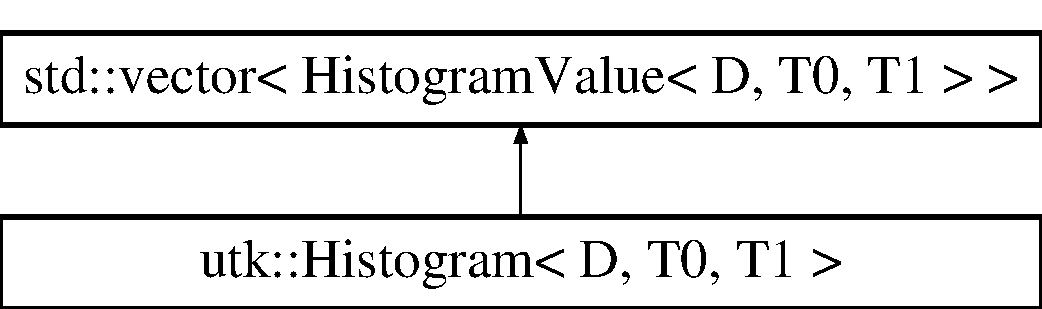
\includegraphics[height=2.000000cm]{classutk_1_1Histogram}
\end{center}
\end{figure}
\subsection*{Public Member Functions}
\begin{DoxyCompactItemize}
\item 
\hypertarget{classutk_1_1Histogram_a849d0b6f5d881f518791cd7f2e794018}{bool {\bfseries L2} (const \hyperlink{classutk_1_1Histogram}{Histogram}$<$ D, T0, T1 $>$ \&histo, double \&L2) const }\label{classutk_1_1Histogram_a849d0b6f5d881f518791cd7f2e794018}

\item 
\hypertarget{classutk_1_1Histogram_a9a56bf7a2d5178aef2862eb0c78fe92e}{bool {\bfseries Linf} (const \hyperlink{classutk_1_1Histogram}{Histogram}$<$ D, T0, T1 $>$ \&histo, double \&Linf) const }\label{classutk_1_1Histogram_a9a56bf7a2d5178aef2862eb0c78fe92e}

\item 
\hypertarget{classutk_1_1Histogram_a3bf6f55d31e01d4406919fe5a93ba521}{\hyperlink{classutk_1_1Histogram}{Histogram}$<$ D, T0, T1 $>$ {\bfseries operator-\/} (const \hyperlink{classutk_1_1Histogram}{Histogram}$<$ D, T0, T1 $>$ \&histo) const }\label{classutk_1_1Histogram_a3bf6f55d31e01d4406919fe5a93ba521}

\end{DoxyCompactItemize}


\subsection{Detailed Description}
\subsubsection*{template$<$uint D, typename T0, typename T1$>$class utk\-::\-Histogram$<$ D, T0, T1 $>$}

A D-\/dimensional histogram. 

This class is mostly used to represent the P\-C\-F of a sampling pattern (1\-D histogram), its fourier spectrum (2\-D histogram), or its spectral radial average (1\-D histogram). 

The documentation for this class was generated from the following file\-:\begin{DoxyCompactItemize}
\item 
src/pointsets/Histogram.\-hpp\end{DoxyCompactItemize}

\hypertarget{classutk_1_1HistogramReader}{\section{utk\-:\-:Histogram\-Reader$<$ D, T0, T1 $>$ Class Template Reference}
\label{classutk_1_1HistogramReader}\index{utk\-::\-Histogram\-Reader$<$ D, T0, T1 $>$@{utk\-::\-Histogram\-Reader$<$ D, T0, T1 $>$}}
}


Fills an instance of the \hyperlink{classutk_1_1Histogram}{Histogram} class from an ascii file.  




{\ttfamily \#include $<$histogram\-I\-O.\-hpp$>$}

\subsection*{Public Member Functions}
\begin{DoxyCompactItemize}
\item 
\hypertarget{classutk_1_1HistogramReader_a1a2684f4786dc20a7ba8d698e5898f4c}{bool {\bfseries open} (const std\-::string arg\-\_\-filename)}\label{classutk_1_1HistogramReader_a1a2684f4786dc20a7ba8d698e5898f4c}

\item 
\hypertarget{classutk_1_1HistogramReader_afd1ec63b0aba6a325af298b573b83659}{virtual bool {\bfseries read\-Histogram} (\hyperlink{classutk_1_1Histogram}{Histogram}$<$ D, T0, T1 $>$ \&arg\-\_\-histo)}\label{classutk_1_1HistogramReader_afd1ec63b0aba6a325af298b573b83659}

\item 
\hypertarget{classutk_1_1HistogramReader_a56421b96b8878fe25e44cc18a0443a1f}{void {\bfseries close} ()}\label{classutk_1_1HistogramReader_a56421b96b8878fe25e44cc18a0443a1f}

\end{DoxyCompactItemize}


\subsection{Detailed Description}
\subsubsection*{template$<$uint D, typename T0, typename T1$>$class utk\-::\-Histogram\-Reader$<$ D, T0, T1 $>$}

Fills an instance of the \hyperlink{classutk_1_1Histogram}{Histogram} class from an ascii file. 

The documentation for this class was generated from the following file\-:\begin{DoxyCompactItemize}
\item 
src/io/histogram\-I\-O.\-hpp\end{DoxyCompactItemize}

\hypertarget{classutk_1_1HistogramWriter}{\section{utk\-:\-:Histogram\-Writer$<$ D, T0, T1 $>$ Class Template Reference}
\label{classutk_1_1HistogramWriter}\index{utk\-::\-Histogram\-Writer$<$ D, T0, T1 $>$@{utk\-::\-Histogram\-Writer$<$ D, T0, T1 $>$}}
}


Outputs an histogram in ascii mode.  




{\ttfamily \#include $<$histogram\-I\-O.\-hpp$>$}

\subsection*{Public Member Functions}
\begin{DoxyCompactItemize}
\item 
\hypertarget{classutk_1_1HistogramWriter_aa95d9a7349a6a873f980f1414fece8ee}{bool {\bfseries open} (const std\-::string arg\-\_\-filename)}\label{classutk_1_1HistogramWriter_aa95d9a7349a6a873f980f1414fece8ee}

\item 
\hypertarget{classutk_1_1HistogramWriter_ab13e62c1373e6eaa8c9382552a9119b1}{virtual bool {\bfseries write\-Histogram} (const \hyperlink{classutk_1_1Histogram}{Histogram}$<$ D, T0, T1 $>$ \&arg\-\_\-histo)}\label{classutk_1_1HistogramWriter_ab13e62c1373e6eaa8c9382552a9119b1}

\item 
\hypertarget{classutk_1_1HistogramWriter_af99a6ab66dd2eb92d97a26a1a857208c}{void {\bfseries close} ()}\label{classutk_1_1HistogramWriter_af99a6ab66dd2eb92d97a26a1a857208c}

\end{DoxyCompactItemize}


\subsection{Detailed Description}
\subsubsection*{template$<$uint D, typename T0, typename T1$>$class utk\-::\-Histogram\-Writer$<$ D, T0, T1 $>$}

Outputs an histogram in ascii mode. 

The documentation for this class was generated from the following file\-:\begin{DoxyCompactItemize}
\item 
src/io/histogram\-I\-O.\-hpp\end{DoxyCompactItemize}

\hypertarget{classutk_1_1Point}{\section{utk\-:\-:Point$<$ D, T $>$ Class Template Reference}
\label{classutk_1_1Point}\index{utk\-::\-Point$<$ D, T $>$@{utk\-::\-Point$<$ D, T $>$}}
}


A D-\/dimensional sample with coordinates of type T.  




{\ttfamily \#include $<$Point.\-hpp$>$}

\subsection*{Public Member Functions}
\begin{DoxyCompactItemize}
\item 
\hypertarget{classutk_1_1Point_a009dae3aa21d34d2a553ca15f12ee742}{{\bfseries Point} (const T \&f)}\label{classutk_1_1Point_a009dae3aa21d34d2a553ca15f12ee742}

\item 
\hypertarget{classutk_1_1Point_a027e496c55b33346694b8eb3d253febc}{{\bfseries Point} (const T val\mbox{[}D\mbox{]})}\label{classutk_1_1Point_a027e496c55b33346694b8eb3d253febc}

\item 
\hypertarget{classutk_1_1Point_ae4d29aeba9f6adde7b8ca2153eee4354}{{\bfseries Point} (const T \&i, const T \&j)}\label{classutk_1_1Point_ae4d29aeba9f6adde7b8ca2153eee4354}

\item 
\hypertarget{classutk_1_1Point_a09a47085bfa534f5e955bd91421608ac}{{\bfseries Point} (const T \&i, const T \&j, const T \&k)}\label{classutk_1_1Point_a09a47085bfa534f5e955bd91421608ac}

\item 
\hypertarget{classutk_1_1Point_ada888533453661263b81bf4077ef3d82}{{\bfseries Point} (const T \&i, const T \&j, const T \&k, const T \&l)}\label{classutk_1_1Point_ada888533453661263b81bf4077ef3d82}

\item 
\hypertarget{classutk_1_1Point_aac498658f758e4681e7c8aabc720f456}{{\bfseries Point} (const \hyperlink{classutk_1_1Point}{Point}$<$ D, T $>$ \&arg\-\_\-pt)}\label{classutk_1_1Point_aac498658f758e4681e7c8aabc720f456}

\item 
\hypertarget{classutk_1_1Point_a21dfa1b8720040d2c1fd5afb33a23579}{void {\bfseries pos} (const \hyperlink{classutk_1_1Vector}{Vector}$<$ D, T $>$ \&arg\-\_\-pos)}\label{classutk_1_1Point_a21dfa1b8720040d2c1fd5afb33a23579}

\item 
\hypertarget{classutk_1_1Point_a7a8ced7f77049fac274e496e69edc2cd}{\hyperlink{classutk_1_1Vector}{Vector}$<$ D, T $>$ \& {\bfseries pos} ()}\label{classutk_1_1Point_a7a8ced7f77049fac274e496e69edc2cd}

\item 
\hypertarget{classutk_1_1Point_a093be2f178e1b34e1ec026801cfb0b2f}{\hyperlink{classutk_1_1Vector}{Vector}$<$ D, T $>$ {\bfseries pos} () const }\label{classutk_1_1Point_a093be2f178e1b34e1ec026801cfb0b2f}

\item 
\hypertarget{classutk_1_1Point_a39138843aa2dc8e07f1a9b7b9e3c7a25}{bool {\bfseries operator==} (const \hyperlink{classutk_1_1Point}{Point}$<$ D, T $>$ arg\-\_\-pt) const }\label{classutk_1_1Point_a39138843aa2dc8e07f1a9b7b9e3c7a25}

\end{DoxyCompactItemize}
\subsection*{Protected Attributes}
\begin{DoxyCompactItemize}
\item 
\hypertarget{classutk_1_1Point_a086a258e984bb353117faf9ea1f4fe78}{\hyperlink{classutk_1_1Vector}{Vector}$<$ D, T $>$ {\bfseries m\-\_\-pos}}\label{classutk_1_1Point_a086a258e984bb353117faf9ea1f4fe78}

\end{DoxyCompactItemize}


\subsection{Detailed Description}
\subsubsection*{template$<$unsigned int D, typename T$>$class utk\-::\-Point$<$ D, T $>$}

A D-\/dimensional sample with coordinates of type T. 

This class includes functions and operator to facilitate the manipulation of points in a point set. 

The documentation for this class was generated from the following file\-:\begin{DoxyCompactItemize}
\item 
src/pointsets/Point.\-hpp\end{DoxyCompactItemize}

\hypertarget{classutk_1_1Pointset}{\section{utk\-:\-:Pointset$<$ D, T, P $>$ Class Template Reference}
\label{classutk_1_1Pointset}\index{utk\-::\-Pointset$<$ D, T, P $>$@{utk\-::\-Pointset$<$ D, T, P $>$}}
}


A vector of D-\/dimensional samples with coordinates of type T.  




{\ttfamily \#include $<$Pointset.\-hpp$>$}

Inheritance diagram for utk\-:\-:Pointset$<$ D, T, P $>$\-:\begin{figure}[H]
\begin{center}
\leavevmode
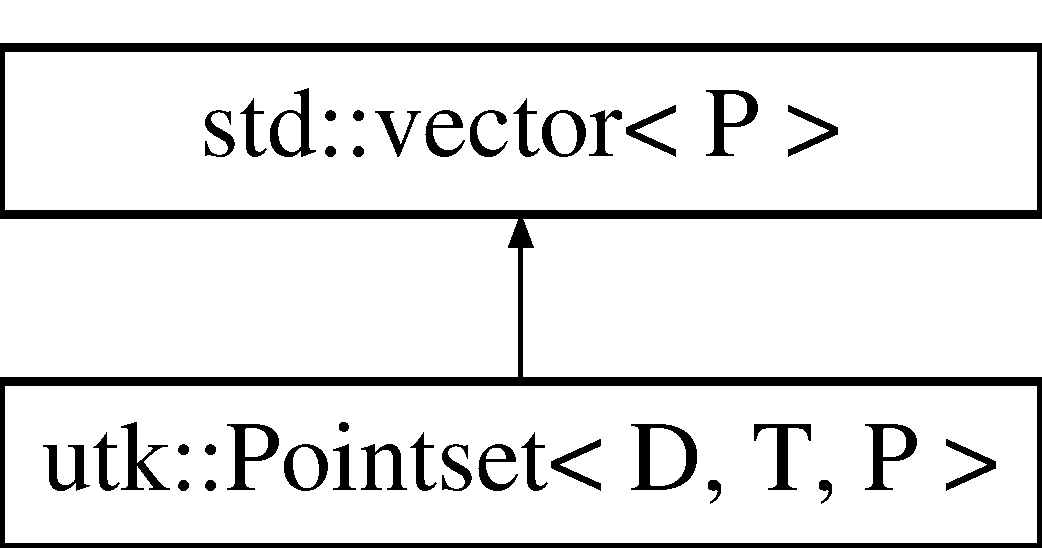
\includegraphics[height=2.000000cm]{classutk_1_1Pointset}
\end{center}
\end{figure}
\subsection*{Public Member Functions}
\begin{DoxyCompactItemize}
\item 
\hypertarget{classutk_1_1Pointset_ac112d4c6ebce6c272d33da5bb57581fe}{double {\bfseries normalize\-Positions} (\hyperlink{classutk_1_1Pointset}{Pointset}$<$ D, double, \hyperlink{classutk_1_1Point}{Point}$<$ D, double $>$ $>$ \&pts2) const }\label{classutk_1_1Pointset_ac112d4c6ebce6c272d33da5bb57581fe}

\item 
\hypertarget{classutk_1_1Pointset_aa7732906b330fcb54e490427452a4255}{void {\bfseries set\-Unit\-Toroidal\-Domain} ()}\label{classutk_1_1Pointset_aa7732906b330fcb54e490427452a4255}

\end{DoxyCompactItemize}
\subsection*{Public Attributes}
\begin{DoxyCompactItemize}
\item 
\hypertarget{classutk_1_1Pointset_ae699b217e6196dd9f235dd98bd78bb56}{\hyperlink{structutk_1_1Domain}{Domain}$<$ P $>$ {\bfseries domain}}\label{classutk_1_1Pointset_ae699b217e6196dd9f235dd98bd78bb56}

\item 
\hypertarget{classutk_1_1Pointset_adc0cf94fe3594f9e61e9580962d66039}{int {\bfseries toricity}}\label{classutk_1_1Pointset_adc0cf94fe3594f9e61e9580962d66039}

\end{DoxyCompactItemize}


\subsection{Detailed Description}
\subsubsection*{template$<$unsigned int D, typename T, typename P$>$class utk\-::\-Pointset$<$ D, T, P $>$}

A vector of D-\/dimensional samples with coordinates of type T. 

This class is used to represent a point set. It is at the core of the U\-T\-K framework and is voluntarily kept as simple as possible and heavily templated for the sake of code modularity. 

The documentation for this class was generated from the following file\-:\begin{DoxyCompactItemize}
\item 
src/pointsets/Pointset.\-hpp\end{DoxyCompactItemize}

\hypertarget{classutk_1_1PointsetIllustrator}{\section{utk\-:\-:Pointset\-Illustrator$<$ D, T, P $>$ Class Template Reference}
\label{classutk_1_1PointsetIllustrator}\index{utk\-::\-Pointset\-Illustrator$<$ D, T, P $>$@{utk\-::\-Pointset\-Illustrator$<$ D, T, P $>$}}
}


Outputs an image from a point set.  




{\ttfamily \#include $<$image\-I\-O.\-hpp$>$}

\subsection*{Public Member Functions}
\begin{DoxyCompactItemize}
\item 
\hypertarget{classutk_1_1PointsetIllustrator_adca3d16b44f95aa34f1ea180b90f5224}{bool {\bfseries open} (const std\-::string arg\-\_\-filename)}\label{classutk_1_1PointsetIllustrator_adca3d16b44f95aa34f1ea180b90f5224}

\item 
\hypertarget{classutk_1_1PointsetIllustrator_a1c452447a54268ed586e5a6885808a1d}{void {\bfseries set\-Color} (float arg\-\_\-r, float arg\-\_\-g, float arg\-\_\-b)}\label{classutk_1_1PointsetIllustrator_a1c452447a54268ed586e5a6885808a1d}

\item 
\hypertarget{classutk_1_1PointsetIllustrator_a841daaa71849c6bf8056e6869039b14b}{void {\bfseries set\-Point\-Radius} (float arg\-\_\-radius)}\label{classutk_1_1PointsetIllustrator_a841daaa71849c6bf8056e6869039b14b}

\item 
\hypertarget{classutk_1_1PointsetIllustrator_ab9fe2e517accfac46b0c84b795e9591e}{void {\bfseries set\-Border\-Size} (double arg\-\_\-bordersize)}\label{classutk_1_1PointsetIllustrator_ab9fe2e517accfac46b0c84b795e9591e}

\item 
\hypertarget{classutk_1_1PointsetIllustrator_a90b527a2ad4ab2e698bf79222fdc8739}{void {\bfseries set\-Font\-Size} (int arg\-\_\-fontsize)}\label{classutk_1_1PointsetIllustrator_a90b527a2ad4ab2e698bf79222fdc8739}

\item 
\hypertarget{classutk_1_1PointsetIllustrator_a84485cb33f00ef582c278bd1dcbbf7cb}{void {\bfseries set\-Numbered} (bool arg\-\_\-numbered)}\label{classutk_1_1PointsetIllustrator_a84485cb33f00ef582c278bd1dcbbf7cb}

\item 
\hypertarget{classutk_1_1PointsetIllustrator_aeac4234f38e73924643c084eb4f21e9f}{void {\bfseries set\-Bounding\-Box} (int arg\-\_\-boundingbox)}\label{classutk_1_1PointsetIllustrator_aeac4234f38e73924643c084eb4f21e9f}

\item 
\hypertarget{classutk_1_1PointsetIllustrator_a78b7e3f89d310a0fd8a89b1ca4a5e972}{void {\bfseries set\-Bounding\-Box\-X} (int arg\-\_\-boundingbox)}\label{classutk_1_1PointsetIllustrator_a78b7e3f89d310a0fd8a89b1ca4a5e972}

\item 
\hypertarget{classutk_1_1PointsetIllustrator_af28eb08c4f523c691e1d796b19a14c24}{void {\bfseries set\-Bounding\-Box\-Y} (int arg\-\_\-boundingbox)}\label{classutk_1_1PointsetIllustrator_af28eb08c4f523c691e1d796b19a14c24}

\item 
\hypertarget{classutk_1_1PointsetIllustrator_ae94d47180198d9309c55ba3968a72384}{void {\bfseries set\-Tiled} (bool arg\-\_\-tiled)}\label{classutk_1_1PointsetIllustrator_ae94d47180198d9309c55ba3968a72384}

\item 
\hypertarget{classutk_1_1PointsetIllustrator_a5dfd201a1a0ed931f2e4e8d35386f2fb}{void {\bfseries set\-Projection} (unsigned int arg\-\_\-dimension\-\_\-0, unsigned int arg\-\_\-dimension\-\_\-1)}\label{classutk_1_1PointsetIllustrator_a5dfd201a1a0ed931f2e4e8d35386f2fb}

\item 
\hypertarget{classutk_1_1PointsetIllustrator_a65f12a0f4c47ed16eebd4c0f2d66fbfb}{virtual bool {\bfseries draw\-Pointset} (\hyperlink{classutk_1_1Pointset}{Pointset}$<$ D, T, P $>$ \&arg\-\_\-pointset)}\label{classutk_1_1PointsetIllustrator_a65f12a0f4c47ed16eebd4c0f2d66fbfb}

\item 
\hypertarget{classutk_1_1PointsetIllustrator_a5b73078e4d190e3c371fb7bb1357e2a6}{virtual bool {\bfseries draw\-Point} (const P \&arg\-\_\-point)}\label{classutk_1_1PointsetIllustrator_a5b73078e4d190e3c371fb7bb1357e2a6}

\item 
\hypertarget{classutk_1_1PointsetIllustrator_a2338f3a939b82cfba03d5f6ee317826e}{virtual bool {\bfseries draw\-Grid} (int arg\-\_\-grid\-\_\-resolution, float linewidth=1, bool dashed=0, std\-::string color=\char`\"{}0.\-75 0.\-75 0.\-75\char`\"{})}\label{classutk_1_1PointsetIllustrator_a2338f3a939b82cfba03d5f6ee317826e}

\item 
\hypertarget{classutk_1_1PointsetIllustrator_af26b4440013fc754bfd98e7754f8374a}{virtual bool {\bfseries draw\-Rectangle} (float x0, float y0, float sx, float sy, float linewidth)}\label{classutk_1_1PointsetIllustrator_af26b4440013fc754bfd98e7754f8374a}

\item 
\hypertarget{classutk_1_1PointsetIllustrator_a4b621c2f56d0640e65f25c4e3e2f4c31}{virtual bool {\bfseries draw\-Circle} (float x0, float y0, float r0, float linewidth)}\label{classutk_1_1PointsetIllustrator_a4b621c2f56d0640e65f25c4e3e2f4c31}

\item 
\hypertarget{classutk_1_1PointsetIllustrator_a18db3dda9ce38834fe719aaa11bb6ff3}{void {\bfseries close} ()}\label{classutk_1_1PointsetIllustrator_a18db3dda9ce38834fe719aaa11bb6ff3}

\end{DoxyCompactItemize}


\subsection{Detailed Description}
\subsubsection*{template$<$unsigned int D, typename T, typename P$>$class utk\-::\-Pointset\-Illustrator$<$ D, T, P $>$}

Outputs an image from a point set. 

The documentation for this class was generated from the following file\-:\begin{DoxyCompactItemize}
\item 
src/io/image\-I\-O.\-hpp\end{DoxyCompactItemize}

\hypertarget{classutk_1_1PointsetReader}{\section{utk\-:\-:Pointset\-Reader$<$ D, T, P $>$ Class Template Reference}
\label{classutk_1_1PointsetReader}\index{utk\-::\-Pointset\-Reader$<$ D, T, P $>$@{utk\-::\-Pointset\-Reader$<$ D, T, P $>$}}
}


Fills an instance of the \hyperlink{classutk_1_1Pointset}{Pointset} class from an ascii or binary file.  




{\ttfamily \#include $<$file\-I\-O.\-hpp$>$}

\subsection*{Public Member Functions}
\begin{DoxyCompactItemize}
\item 
\hypertarget{classutk_1_1PointsetReader_aa2f5cf05ce69982d8cab7353c981bb3b}{bool {\bfseries open} (const std\-::string arg\-\_\-filename)}\label{classutk_1_1PointsetReader_aa2f5cf05ce69982d8cab7353c981bb3b}

\item 
\hypertarget{classutk_1_1PointsetReader_a2c0646b6433cf2896c001015a6544102}{virtual bool {\bfseries read\-Pointset} (\hyperlink{classutk_1_1Pointset}{Pointset}$<$ D, T, P $>$ \&arg\-\_\-pointset)}\label{classutk_1_1PointsetReader_a2c0646b6433cf2896c001015a6544102}

\item 
\hypertarget{classutk_1_1PointsetReader_a481325b7ec8e5c2ab86b03ef79f18ee3}{void {\bfseries close} ()}\label{classutk_1_1PointsetReader_a481325b7ec8e5c2ab86b03ef79f18ee3}

\end{DoxyCompactItemize}


\subsection{Detailed Description}
\subsubsection*{template$<$unsigned int D, typename T, typename P$>$class utk\-::\-Pointset\-Reader$<$ D, T, P $>$}

Fills an instance of the \hyperlink{classutk_1_1Pointset}{Pointset} class from an ascii or binary file. 

The documentation for this class was generated from the following file\-:\begin{DoxyCompactItemize}
\item 
src/io/file\-I\-O.\-hpp\end{DoxyCompactItemize}

\hypertarget{classutk_1_1PointsetWriter}{\section{utk\-:\-:Pointset\-Writer$<$ D, T, P $>$ Class Template Reference}
\label{classutk_1_1PointsetWriter}\index{utk\-::\-Pointset\-Writer$<$ D, T, P $>$@{utk\-::\-Pointset\-Writer$<$ D, T, P $>$}}
}


Outputs an ascii or binary point set.  




{\ttfamily \#include $<$file\-I\-O.\-hpp$>$}

\subsection*{Public Member Functions}
\begin{DoxyCompactItemize}
\item 
\hypertarget{classutk_1_1PointsetWriter_ae5bb1fee762747382d5c17d537212c8b}{bool {\bfseries open} (const std\-::string arg\-\_\-filename)}\label{classutk_1_1PointsetWriter_ae5bb1fee762747382d5c17d537212c8b}

\item 
\hypertarget{classutk_1_1PointsetWriter_ae89f494289b002d9cfc3bb57d734e1d4}{virtual bool {\bfseries write\-Pointset} (\hyperlink{classutk_1_1Pointset}{Pointset}$<$ D, T, P $>$ \&arg\-\_\-pointset)}\label{classutk_1_1PointsetWriter_ae89f494289b002d9cfc3bb57d734e1d4}

\item 
\hypertarget{classutk_1_1PointsetWriter_a0ab938eebea5b1906ebb2677ca203637}{void {\bfseries close} ()}\label{classutk_1_1PointsetWriter_a0ab938eebea5b1906ebb2677ca203637}

\end{DoxyCompactItemize}


\subsection{Detailed Description}
\subsubsection*{template$<$unsigned int D, typename T, typename P$>$class utk\-::\-Pointset\-Writer$<$ D, T, P $>$}

Outputs an ascii or binary point set. 

The documentation for this class was generated from the following file\-:\begin{DoxyCompactItemize}
\item 
src/io/file\-I\-O.\-hpp\end{DoxyCompactItemize}

\hypertarget{classutk_1_1Vector}{\section{utk\-:\-:Vector$<$ D, T $>$ Class Template Reference}
\label{classutk_1_1Vector}\index{utk\-::\-Vector$<$ D, T $>$@{utk\-::\-Vector$<$ D, T $>$}}
}


A D-\/dimensional vector of values of type T.  




{\ttfamily \#include $<$Vector.\-hpp$>$}

\subsection*{Public Member Functions}
\begin{DoxyCompactItemize}
\item 
\hypertarget{classutk_1_1Vector_af835ce1423f91fc3368a8ff1056d2149}{{\bfseries Vector} (T f=0)}\label{classutk_1_1Vector_af835ce1423f91fc3368a8ff1056d2149}

\item 
\hypertarget{classutk_1_1Vector_aa18e15a91b22df08ccf3ab81a7c509b0}{{\bfseries Vector} (const T val\mbox{[}D\mbox{]})}\label{classutk_1_1Vector_aa18e15a91b22df08ccf3ab81a7c509b0}

\item 
\hypertarget{classutk_1_1Vector_a4ef62c8a3d99c1267bc337832db01fdc}{{\bfseries Vector} (T i, T j, T k=0, T l=0)}\label{classutk_1_1Vector_a4ef62c8a3d99c1267bc337832db01fdc}

\item 
\hypertarget{classutk_1_1Vector_a353195f5d9a7f28178387dc96056387f}{{\bfseries Vector} (const \hyperlink{classutk_1_1Vector}{Vector}$<$ D, T $>$ \&arg\-\_\-v)}\label{classutk_1_1Vector_a353195f5d9a7f28178387dc96056387f}

\item 
\hypertarget{classutk_1_1Vector_a431fcd5a1eb0ded1c89fcf1785378d16}{\hyperlink{classutk_1_1Vector}{Vector}$<$ D, T $>$ {\bfseries operator+} (const \hyperlink{classutk_1_1Vector}{Vector}$<$ D, T $>$ \&v) const }\label{classutk_1_1Vector_a431fcd5a1eb0ded1c89fcf1785378d16}

\item 
\hypertarget{classutk_1_1Vector_a29574556883ea1d820c84e3aa0720d7f}{\hyperlink{classutk_1_1Vector}{Vector}$<$ D, T $>$ \& {\bfseries operator+=} (const \hyperlink{classutk_1_1Vector}{Vector}$<$ D, T $>$ \&v)}\label{classutk_1_1Vector_a29574556883ea1d820c84e3aa0720d7f}

\item 
\hypertarget{classutk_1_1Vector_af9a570ccfc436ca299d87c7b85ad88d7}{\hyperlink{classutk_1_1Vector}{Vector}$<$ D, T $>$ {\bfseries operator-\/} (const \hyperlink{classutk_1_1Vector}{Vector}$<$ D, T $>$ \&v) const }\label{classutk_1_1Vector_af9a570ccfc436ca299d87c7b85ad88d7}

\item 
\hypertarget{classutk_1_1Vector_a45d6fb956fcab8d580e4a9700cf344c8}{\hyperlink{classutk_1_1Vector}{Vector}$<$ D, T $>$ \& {\bfseries operator-\/=} (const \hyperlink{classutk_1_1Vector}{Vector}$<$ D, T $>$ \&v)}\label{classutk_1_1Vector_a45d6fb956fcab8d580e4a9700cf344c8}

\item 
\hypertarget{classutk_1_1Vector_ad1e177c46e7db4795f13b702b158cd02}{\hyperlink{classutk_1_1Vector}{Vector}$<$ D, T $>$ {\bfseries operator-\/} () const }\label{classutk_1_1Vector_ad1e177c46e7db4795f13b702b158cd02}

\item 
\hypertarget{classutk_1_1Vector_abfbc8ea9192e67c9ca0e9c6c6585a44e}{\hyperlink{classutk_1_1Vector}{Vector}$<$ D, T $>$ {\bfseries operator$\ast$} (double f) const }\label{classutk_1_1Vector_abfbc8ea9192e67c9ca0e9c6c6585a44e}

\item 
\hypertarget{classutk_1_1Vector_ab7856bb07d25997d8e632914e8fff1d0}{\hyperlink{classutk_1_1Vector}{Vector}$<$ D, T $>$ \& {\bfseries operator$\ast$=} (double f)}\label{classutk_1_1Vector_ab7856bb07d25997d8e632914e8fff1d0}

\item 
\hypertarget{classutk_1_1Vector_afc08f6be481e40fda0dc5b2d797984fc}{\hyperlink{classutk_1_1Vector}{Vector}$<$ D, T $>$ {\bfseries operator$\ast$} (const \hyperlink{classutk_1_1Vector}{Vector}$<$ D, T $>$ \&v) const }\label{classutk_1_1Vector_afc08f6be481e40fda0dc5b2d797984fc}

\item 
\hypertarget{classutk_1_1Vector_af3268322de09c7a1ed580a63beee0506}{\hyperlink{classutk_1_1Vector}{Vector}$<$ D, T $>$ \& {\bfseries operator$\ast$=} (const \hyperlink{classutk_1_1Vector}{Vector}$<$ D, T $>$ \&v)}\label{classutk_1_1Vector_af3268322de09c7a1ed580a63beee0506}

\item 
\hypertarget{classutk_1_1Vector_a07598b25983aa04da007659f4bf33707}{\hyperlink{classutk_1_1Vector}{Vector}$<$ D, T $>$ {\bfseries operator/} (double f) const }\label{classutk_1_1Vector_a07598b25983aa04da007659f4bf33707}

\item 
\hypertarget{classutk_1_1Vector_a7051861964e2082701faab81b68534e1}{\hyperlink{classutk_1_1Vector}{Vector}$<$ D, T $>$ \& {\bfseries operator/=} (double f)}\label{classutk_1_1Vector_a7051861964e2082701faab81b68534e1}

\item 
\hypertarget{classutk_1_1Vector_abf49cd7c3a7be2631cdd7c3cf9647f13}{T {\bfseries operator\mbox{[}$\,$\mbox{]}} (uint i) const }\label{classutk_1_1Vector_abf49cd7c3a7be2631cdd7c3cf9647f13}

\item 
\hypertarget{classutk_1_1Vector_ac159eb83f7b44815bbe50c52441ca89b}{T \& {\bfseries operator\mbox{[}$\,$\mbox{]}} (uint i)}\label{classutk_1_1Vector_ac159eb83f7b44815bbe50c52441ca89b}

\item 
\hypertarget{classutk_1_1Vector_a1f72121da7293960e0148ec634e5f811}{void {\bfseries set\-All} (T d)}\label{classutk_1_1Vector_a1f72121da7293960e0148ec634e5f811}

\item 
\hypertarget{classutk_1_1Vector_acbbbec5d3c3515733354304774d1abe3}{void {\bfseries set} (uint i, T d)}\label{classutk_1_1Vector_acbbbec5d3c3515733354304774d1abe3}

\item 
\hypertarget{classutk_1_1Vector_aaca32a1fc634b1cf97020e7f7d02b315}{bool {\bfseries operator$>$} (const \hyperlink{classutk_1_1Vector}{Vector}$<$ D, T $>$ \&v)}\label{classutk_1_1Vector_aaca32a1fc634b1cf97020e7f7d02b315}

\item 
\hypertarget{classutk_1_1Vector_ade3523340d345bab3c167fbc7f65694f}{bool {\bfseries operator$<$} (const \hyperlink{classutk_1_1Vector}{Vector}$<$ D, T $>$ \&v)}\label{classutk_1_1Vector_ade3523340d345bab3c167fbc7f65694f}

\item 
\hypertarget{classutk_1_1Vector_aa442c06f51432af64ade91d99911a43e}{bool {\bfseries operator$>$=} (const \hyperlink{classutk_1_1Vector}{Vector}$<$ D, T $>$ \&v)}\label{classutk_1_1Vector_aa442c06f51432af64ade91d99911a43e}

\item 
\hypertarget{classutk_1_1Vector_a1410ccfeecd43e0217f5ada6dcbad7be}{bool {\bfseries operator$<$=} (const \hyperlink{classutk_1_1Vector}{Vector}$<$ D, T $>$ \&v)}\label{classutk_1_1Vector_a1410ccfeecd43e0217f5ada6dcbad7be}

\item 
\hypertarget{classutk_1_1Vector_a8b1b3c2370ace9d7ff262af5e5eeece7}{bool {\bfseries operator==} (const \hyperlink{classutk_1_1Vector}{Vector}$<$ D, T $>$ \&v) const }\label{classutk_1_1Vector_a8b1b3c2370ace9d7ff262af5e5eeece7}

\item 
\hypertarget{classutk_1_1Vector_abeef808ef700ab49a4323485a178eeed}{bool {\bfseries operator!=} (const \hyperlink{classutk_1_1Vector}{Vector}$<$ D, T $>$ \&v)}\label{classutk_1_1Vector_abeef808ef700ab49a4323485a178eeed}

\item 
\hypertarget{classutk_1_1Vector_abcc8ed414ad75a2696763d5c1bde11d2}{void {\bfseries operator=} (const \hyperlink{classutk_1_1Vector}{Vector}$<$ D, T $>$ \&arg\-\_\-v)}\label{classutk_1_1Vector_abcc8ed414ad75a2696763d5c1bde11d2}

\item 
\hypertarget{classutk_1_1Vector_a4a3fa93c76946b4a8a373377e5381d54}{double {\bfseries length\-Square} () const }\label{classutk_1_1Vector_a4a3fa93c76946b4a8a373377e5381d54}

\item 
\hypertarget{classutk_1_1Vector_adbe9844cf6fb801b9ce6d2a27a82b167}{double {\bfseries length} () const }\label{classutk_1_1Vector_adbe9844cf6fb801b9ce6d2a27a82b167}

\item 
\hypertarget{classutk_1_1Vector_ac585d9dc035cc5993980c19777b01235}{unsigned int {\bfseries nb\-Coord} ()}\label{classutk_1_1Vector_ac585d9dc035cc5993980c19777b01235}

\end{DoxyCompactItemize}
\subsection*{Public Attributes}
\begin{DoxyCompactItemize}
\item 
\hypertarget{classutk_1_1Vector_a03999540f5928420c3dd36898313b546}{T {\bfseries data} \mbox{[}D\mbox{]}}\label{classutk_1_1Vector_a03999540f5928420c3dd36898313b546}

\end{DoxyCompactItemize}


\subsection{Detailed Description}
\subsubsection*{template$<$uint D, typename T$>$class utk\-::\-Vector$<$ D, T $>$}

A D-\/dimensional vector of values of type T. 

The documentation for this class was generated from the following file\-:\begin{DoxyCompactItemize}
\item 
src/pointsets/Vector.\-hpp\end{DoxyCompactItemize}

%--- End generated contents ---

% Index
\newpage
\phantomsection
\addcontentsline{toc}{chapter}{Index}
\printindex

\end{document}
